 \documentclass[book.tex]{subfiles}
\begin{document}

\section{Tricks}

This section describes random tricks used to speed up rendering. 




\subsection{Bouncing Flower}
When Keen throws a flower it bounces of the walls. For flat walls and floors the bounce can be easily calculated by reversing either the x-speed (for vertical walls) or y-speed (for horizontal walls). It becomes more complicated for slopes. Making an accurate calculation of the bounce on a slope requires expensive \cw{cos} and \cw{sin} methods. \\
\par
Instead, the game used a simple algorithm that approximates the angle to either 22$^{\circ}$, 45$^{\circ}$ or 90$^{\circ}$. Based on the ratio between the x- and y-speed it calculates the resulting speed and corresponding angle. Notice that for higher precision the speed is multiplied with 256.\\
\par
\begin{figure}[H]
\centering
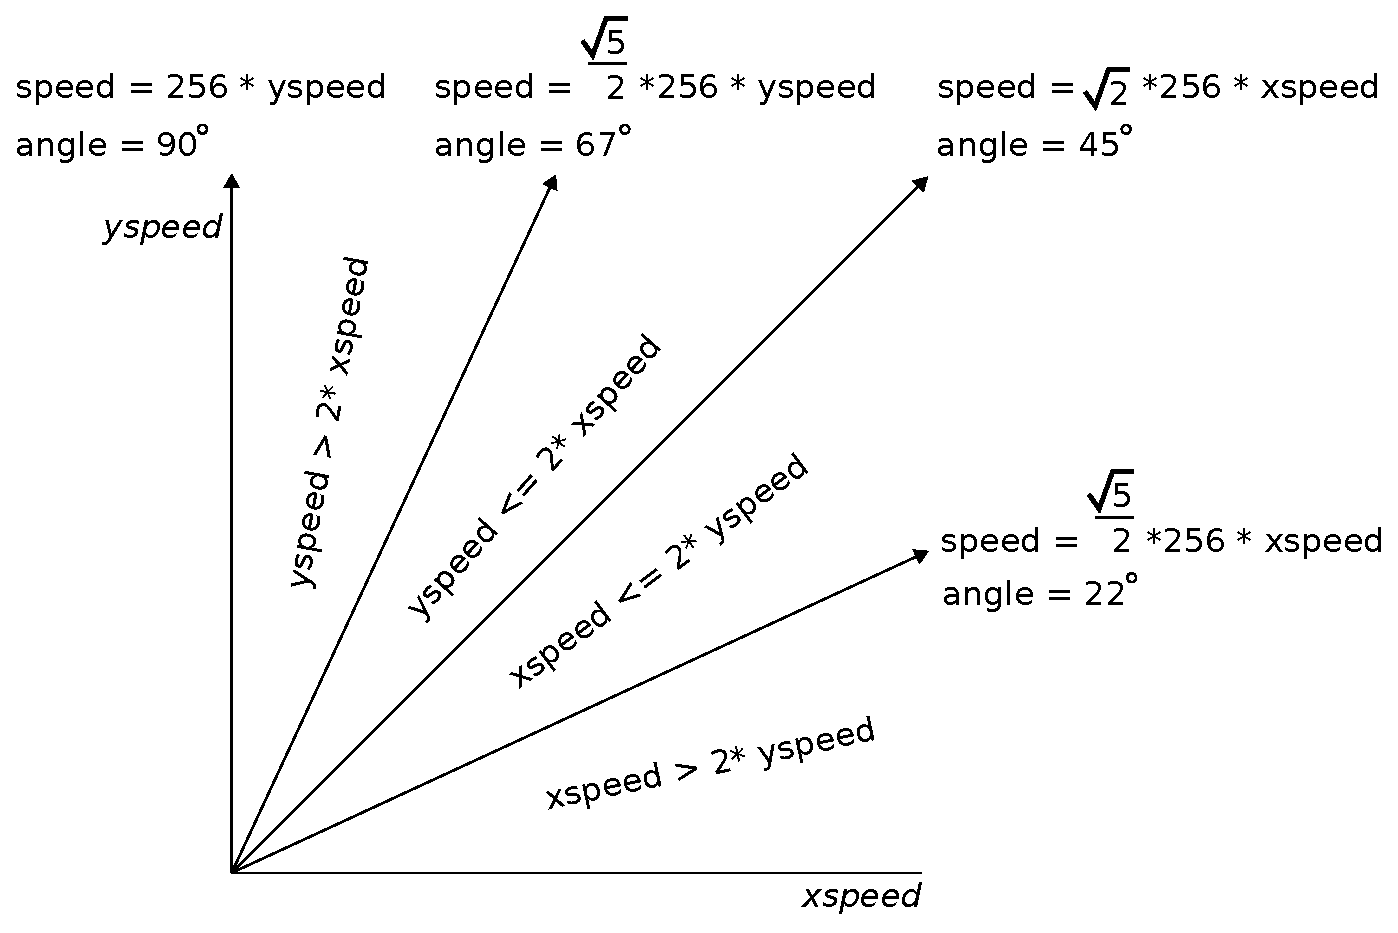
\includegraphics[width=0.8\textwidth]{imgs/drawings/angle.eps}
\label{fig:angles}
\end{figure}
\par

For each combination of the eight type of slopes (Figure \ref{fig:walltype}) and incoming angle, the corresponding bounce angle is calculated using a simple lookup table.\\

\par
\begin{minipage}{\textwidth}
  \lstinputlisting[language=C]{code/bounceangle_lookup.c}
\end{minipage}
\label{wallclip_array}
\par

The value in the table refers to the corresponding bounce angle calculation. As example, waltype 3 with incoming angle of 22$^{\circ}$, results in bounce calculation case 5.

\par
\begin{figure}[H]
\centering
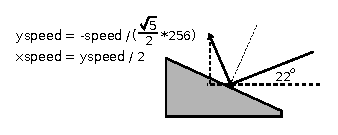
\includegraphics[width=0.7\textwidth]{imgs/drawings/bounce_angle.eps}
\caption{Walltype 3 with incoming angle of 22$^{\circ}$ (angle=0).}
\label{fig:bounce_angles}
\end{figure}
\par

\par
\begin{minipage}{\textwidth}
  \lstinputlisting[language=C]{code/angle.c}
\end{minipage}
\label{wallclip_array}
\par

Notice that in several cases the bounce angle is not following the laws of physics. As example, for an incoming angle of 22$^{\circ}$ on a 45$^{\circ}$ slope the bounce angle is 90$^{\circ}$, instead of 67$^{\circ}$.
\par
\begin{figure}[H]
\centering
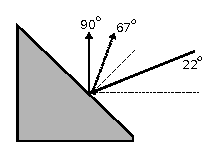
\includegraphics[width=0.4\textwidth]{imgs/drawings/bounce_physics.eps}
\label{fig:bounce_angles}
\end{figure}
\par



\subsection{Pseudo Random Generator}
Random numbers are necessary for many things during runtime, such as calculating whether an enemy is able to hit the player based on its accuracy. This is achieved with a precalculated pseudo-random series of 256 elements.\\
\par
\begin{minipage}{\textwidth}
\lstinputlisting[language={[x86masm]Assembler}, style=mystyle,basicstyle=\small]{code/rndtable.asm}
\end{minipage}
\par
 Each entry in the array has a dual function. It is an integer within the range [0-255]\footnote{Or at least it was intended to!} and it is also the index of the next entry to fetch for next call. This works overall as a 255 entry chained list. The pseudo-random series is initialized using the current time modulo 256 when the engine starts up.\\

\par
\begin{minipage}{\textwidth}
\lstinputlisting[language={[x86masm]Assembler}]{code/US_InitRndT.asm}
\end{minipage}\\
\par
The random number generator saves the last index in \cw{rndindex}. Upon request for a new number, it simply looks up the new value and updates \cw{rndindex}.
\par
\begin{minipage}{\textwidth}
\lstinputlisting[ language={[x86masm]Assembler}]{code/US_RndT.asm}
\end{minipage}

\subsection{Screen fades}
When a new level is loaded, the screen fades from black to the level.CHECK WHEN SCREEN FADES TO WHITE.
Here it makes use of reassigning the color palette colors. This can easily be done by calling BIOS software interrupt \cw{10h}.\\


\par
\begin{minipage}{\textwidth}
  \lstinputlisting[language={[x86masm]Assembler}]{code/ega_set_palette.c}
\end{minipage}
\label{ega_set_palette}
\par

By calling \cw{\_AX=1002h} the entire palette can be reprogrammed. In this case \cw{ES:BX} points to 17 bytes; an rgbRGB value for each of 16 palette index plus one for the border.\\

\par
Earlier in the hardware chapter, Section \ref{sec:ega_color_palette}, it was explained that most EGA monitors did not support the extended 64-color palette and uses the CGA pin assignment. That means applying "rgbRGB" results in wrong color mapping to the monitor. To better understand this, let's have a look at the pin signals.\\

\begin{figure}[H]
\centering
\begin{table}[H]
\begin{tabularx}{\textwidth}[c]{|>{\hsize=.16\hsize}X |>{\hsize=.42\hsize}X |>{\hsize=.42\hsize}X |}
\hline
\textbf{\color{black} Pin} & \textbf{\color{black} EGA modes} & \textbf{\color{black} CGA modes} \\
\hline
\color{black} 1 & \color{black} Ground &\color{black}Ground \\
\hline
\color{black} 2 & \color{white}\cellcolor{EGA_I_Red} Secondary Red (Intensity) &\color{black}Ground \\
\hline
\color{black} 3 & \color{white}\cellcolor{CGA_Red} Primary Red &\color{white}\cellcolor{CGA_Red} Red \\
\hline
\color{black} 4 & \color{black}\cellcolor{CGA_Green} Primary Green &\color{black}\cellcolor{CGA_Green} Green \\
\hline
\color{black} 5 & \color{white}\cellcolor{CGA_Blue} Primary Blue &\color{white}\cellcolor{CGA_Blue} Blue \\
\hline
\color{black} 6 & \color{black}\cellcolor{EGA_I_Green} Secondary Green (Intensity) &\color{white}\cellcolor{CGA_Dark_Grey}Intensity \\
\hline
\color{black} 7 & \color{white}\cellcolor{EGA_I_Blue} Secondary Blue (Intensity) &\color{black}Reserved \\
\hline
\color{black} 8 & \color{black} Horizontal Sync &\color{black}Horizontal Sync \\
\hline
\color{black} 9 & \color{black} Vertical Sync &\color{black}Vertical Sync \\

\hline

\end{tabularx}
\end{table}
\caption{EGA and CGA DE-9 connector pin signals.}
\label{pin_signals}
 \end{figure}
 
If one assigns the color brown (rgbRGB is \cw{010100b}) to one of the color indexes, the resulting color on the CGA pin assignment is light red; The secondary green pin ("r" in rgbRGB) is mapped to the Intensity pin in CGA mode, which results color red with intensity and not the expected brown color. So mapping the color to one of the indexes is based on "RGB" and setting the Secondary Green ("r") for the  intensity color version. The "b" has no meaning and the "r" (Ground) is normally set to 0.\\

The screen fading is defined with the \cw{colors[7][17]} scheme, where the first 16 columns refer to the color indexes, the last column is the border color. Note that the "b" bit is set for the intensity colors, but this had no effect on the results since the pin is unassigned for CGA.

\begin{figure}[H]
\centering
\setlength{\tabcolsep}{2pt} % set border margin to 3
\small
\begin{tabularx}{\textwidth}[c]{|+X|+X|+X|+X|+X|+X|+X|+X|+X|+X|+X|+X|+X|+X|+X|+X|+X|}  
\hline

\rowcolor{CGA_Black}\rowstyle{\color{white}}  0& 0 & 0 & 0 & 0 & 0 & 0 & 0 & 0 & 0 & 0 & 0 & 0 & 0 & 0 & 0 & 0\\ \hline

\rowcolor{CGA_Black}\rowstyle{\color{white}}  0& 0 & 0 & 0 & 0 & 0 & 0 & 0 & 0 & \cellcolor{CGA_Blue} 1 & \cellcolor{CGA_Green}2 & \cellcolor{CGA_Cyan}3 & \cellcolor{CGA_Red}4 & \cellcolor{CGA_Magenta}5 & \cellcolor{CGA_Brown}6 & \cellcolor{CGA_Light_Grey}7  & 0\\ \hline

\rowcolor{CGA_Black}\rowstyle{\color{white}}  0& 0 & 0 & 0 & 0 & 0 & 0 & 0 & \cellcolor{CGA_Dark_Grey}0x18 & \cellcolor{CGA_Bright_Blue}0x19 & \cellcolor{CGA_Bright_Green}\color{black}0x1a & \cellcolor{CGA_Bright_Cyan}\color{black}0x1b & \cellcolor{CGA_Bright_Red}\color{black}0x1c & \cellcolor{CGA_Bright_Magenta}\color{black}0x1d & \cellcolor{CGA_Bright_Brown}\color{black}0x1e & \cellcolor{CGA_White}\color{black}0x1f & 0\\ \hline

\rowcolor{CGA_Black}\rowstyle{\color{white}}  0& \cellcolor{CGA_Blue} 1 & \cellcolor{CGA_Green}2 & \cellcolor{CGA_Cyan}3 & \cellcolor{CGA_Red}4 & \cellcolor{CGA_Magenta}5 & \cellcolor{CGA_Brown}6 & \cellcolor{CGA_Light_Grey}7 & \cellcolor{CGA_Dark_Grey}0x18 & \cellcolor{CGA_Bright_Blue}0x19 & \cellcolor{CGA_Bright_Green}\color{black}0x1a & \cellcolor{CGA_Bright_Cyan}\color{black}0x1b & \cellcolor{CGA_Bright_Red}\color{black}0x1c & \cellcolor{CGA_Bright_Magenta}\color{black}0x1d & \cellcolor{CGA_Bright_Brown}\color{black}0x1e & \cellcolor{CGA_White}\color{black}0x1f & 0\\ \hline

\rowcolor{CGA_White}\rowstyle{\color{white}}  \cellcolor{CGA_Black}0& \cellcolor{CGA_Blue} 1 & \cellcolor{CGA_Green}2 & \cellcolor{CGA_Cyan}3 & \cellcolor{CGA_Red}4 & \cellcolor{CGA_Magenta}5 & \cellcolor{CGA_Brown}6 & \cellcolor{CGA_Light_Grey}7 & \color{black}0x1f & \color{black}0x1f & \color{black}0x1f & \color{black}0x1f & \color{black}0x1f & \color{black}0x1f & \color{black}0x1f & \color{black}0x1f & \cellcolor{CGA_Black}0\\ \hline

\rowcolor{CGA_White}\rowstyle{\color{black}}  0x1f& 0x1f & 0x1f & 0x1f & 0x1f & 0x1f & 0x1f & 0x1f & 0x1f & 0x1f & 0x1f & 0x1f & 0x1f & 0x1f & 0x1f & 0x1f & 0x1f\\ \hline

\end{tabularx}\\
\setlength{\tabcolsep}{6pt} % reset border margin
\caption{Color fading table.}
\end{figure}

Fading the screen is rather straight forward.\\
\par
\begin{minipage}{\textwidth}
  \lstinputlisting[language=C]{code/ega_fade_in.c}
\end{minipage}
\label{ega_fade_in}
\par


\end{document}



